\chapter{Vendetta, Honour and the Mafia}
\label{ch:gould}

\section{Order without courts}

Courts are one solution to the problem of social order. When a person is wronged, the state hears the claim, finds the facts and enforces a remedy. Where courts are absent, distant, slow or untrusted, people find other solutions. Families avenge their members. Communities ostracise wrongdoers. Merchants trade only with those whose reputations they know. Private organisations sell protection. These alternatives are not merely primitive versions of law. They are institutions with their own logic, and that logic is in large part a logic of signals and inference: of revealing and learning who can be trusted, who will retaliate and who is strong.\index{social order}

This chapter examines two bodies of work on order without effective state courts. Roger Gould, a sociologist who taught at the University of Chicago and Yale before his early death in 2002, studied vendetta in nineteenth century Corsica and developed a general theory of interpersonal conflict \citep{gould2000,gould2003}. Diego Gambetta studied the Sicilian mafia as an industry selling private protection \citep{gambetta1993}. Gould's empirical work was on Corsica, the French Mediterranean island whose clan structure, honour culture and weak state presence closely resembled those of Sicily, and Gambetta's on Sicily itself. Together they show how Bayesian ideas about signals, reputations and uncertain rank illuminate societies where the courts do not settle disputes.

\section{Gould on Corsican vendetta}

\subsection{The puzzle}

Corsica was famous in the nineteenth century for vendetta. Novels such as Prosper M\'erim\'ee's \emph{Colomba} portrayed a society in which families were bound by an iron duty to avenge their dead, and in which feuds persisted for generations. Social scientists attributed vendetta to a culture of collective honour and collective responsibility: an injury to one was an injury to the whole kin group, and any member of the offender's group was a legitimate target.\index{Corsica}\index{vendetta}

Gould tested this account against evidence. He used French court records of violent incidents in Corsica in the second half of the nineteenth century, which recorded the relationships between offenders, victims and others involved \citep{gould2000}. From these he could estimate how often killings were avenged, what predicted revenge, and who was targeted.

\subsection{Findings}

Gould's findings contradicted the cultural account in several respects. Vengeance was rare: most killings were not avenged at all. When vengeance occurred, it typically followed incidents in which the original attack had involved collaboration among several members of the offender's group, or violence against people who were not parties to the dispute. Vengeance rarely extended beyond the nuclear family; when it did, correspondingly distant kin of the victim acted as avengers. And the targets of revenge were selected on the basis of specific acts of solidarity with the original offender, such as participating in the attack or sheltering the killer, not on abstract collective responsibility.

Gould concluded that vengeance was a purposeful sanction against collective aggression, calibrated to demonstrate that the aggrieved family's cohesiveness matched that displayed by the offender's group. Vendettas were strategic yet altruistic acts: strategic because they responded to specific displays and were scaled to them, altruistic because the avenger bore risk on behalf of the group.

\subsection{A Bayesian reading}

Gould's account is naturally expressed in terms of signals. When a group acts together in violence, it reveals its cohesion: its members are willing to bear risk for each other. Other groups update their beliefs about the group's strength. A family that is attacked by a cohesive group and does not respond reveals, or is taken to reveal, that it lacks the cohesion to defend itself, and its posterior strength in the eyes of others falls. Further aggression against it becomes more attractive. Revenge restores the family's reputation by matching the signal: it demonstrates cohesion of the same degree.\index{costly signalling}

When the original attack was by a single individual acting alone, it revealed nothing about the cohesion of his group, and failure to respond carried no reputational cost to the victim's family as a group. Revenge was then unnecessary from the point of view of reputation, and the costs of violence, including prosecution by the French state, dominated. This would explain why revenge was rare after individual attacks and more common after collective ones. Figure~\ref{fig:vendetta} illustrates the pattern with a stylised model in which the probability of revenge rises with the size of the victim's kin group and with the degree of collaboration in the original attack.

\begin{figure}[t]
\centering
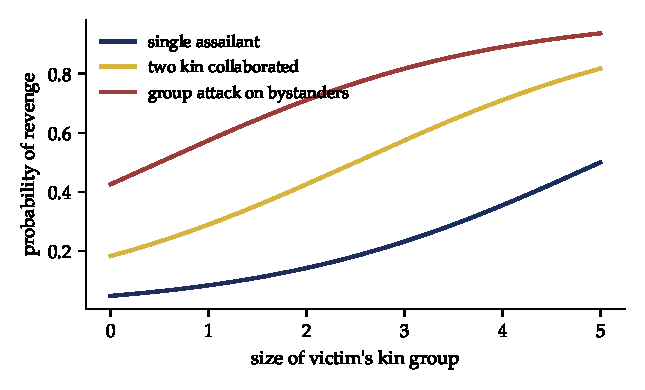
\includegraphics[width=\linewidth]{fig_vendetta}
\caption{A stylised model of the probability of revenge as a function of the size of the victim's kin group, for three kinds of original attack: a single assailant, two kin collaborating, and a group attack on bystanders. Collective attacks and attacks on bystanders, which signal the offender group's cohesion, make revenge more likely. Illustrative, not estimated from Gould's data.}
\label{fig:vendetta}
\end{figure}

The selection of targets follows the same logic. An avenger who killed an arbitrary member of the offender's kin would signal only a willingness to kill. One who killed a person who had displayed solidarity with the offender, by joining the attack or hiding him, signalled that the family would respond precisely to acts of solidarity, raising the cost of such acts in the future. Revenge was a sanction, and sanctions deter only if they are targeted at the conduct to be deterred.

\subsection{Vendetta and the state}

Gould's Corsica was not stateless. It was a French department with courts, prosecutors and gendarmes, and the records he used were produced by them. But the state's reach was limited, its legitimacy contested, and its procedures slow. Families could not rely on the courts to protect them or to deter aggressors. Vendetta coexisted with prosecution: an avenger might be prosecuted, and the prosecution might itself be part of the feud, as families used the courts against each other. Stephen Wilson's history of feuding and banditry in nineteenth century Corsica documents the complex interplay between local sanctions and the French judicial system \citep{wilson1988}. The Bayesian point is that families acted on their beliefs about the probability and speed of state enforcement. Where those beliefs were pessimistic, private enforcement filled the gap.

\section{Gould on ambiguous rank}

\subsection{Collision of Wills}

In \emph{Collision of Wills}, published posthumously in 2003, Gould developed a general theory of interpersonal conflict \citep{gould2003}. His central claim was that conflict is most likely in relationships where social rank is ambiguous. In clearly hierarchical relationships, such as parent and young child or employer and employee, each party knows its place, and disputes are resolved by deference. Relationships between equals or near equals are the hardest case, because symmetry leaves relative rank open: neither party has a ready claim to the other's deference. Violence arises when the relative standing of the parties is uncertain or contested: when each believes it is entitled to the other's deference, or when a challenge to one's standing cannot be ignored without accepting a lower position. Gould drew on evidence from homicide records in Corsica and elsewhere, showing that many killings arose from trivial disputes between people of similar status, in which the stakes were not the trivial object but the relationship.\index{Collision of Wills}\index{ambiguous rank}

\subsection{Rank as a posterior}

Gould's theory has a direct Bayesian interpretation. Each party holds a belief about the relative standing of the two: the probability that, if the matter came to a contest, the other would yield. Call party $A$'s belief $p_A$ that $B$ would yield, and $B$'s belief $p_B$ that $A$ would yield. If one belief is near one and the other near zero, so that both agree who would yield, there is no conflict: the subordinate yields. If the beliefs are inconsistent, each expecting the other to yield, both stand firm, and conflict follows. Inconsistent beliefs are most likely when the evidence about relative standing is weak or ambiguous, that is, when the posterior is near one half and each party's prior or interpretation, assumed to be self-serving, pushes it in its own favour.

The same structure appears in theories of litigation and war. Priest and Klein, whose model Chapter~\ref{ch:becker} develops, showed that cases go to trial when the parties' estimates of the outcome diverge, and that this happens most often when the case is close \citep{priest_klein1984}. James Fearon argued that wars occur when states have private information about their strength and incentives to misrepresent it, so that their estimates of the outcome of a war diverge \citep{fearon1995}. Gould's theory applies the same logic to individuals. Conflict is the product of disagreement about a posterior, and disagreement is most likely when the evidence is ambiguous.

The implication for law is that clarifying rights reduces conflict. Where property boundaries are uncertain, disputes are frequent; where they are surveyed and registered, disputes are rare. Where the hierarchy of a workplace is clear, there are fewer personal conflicts than where roles overlap. Legal rules that make entitlements clear move the posterior away from one half and reduce the scope for collisions of will. This is a Bayesian argument for clear rules, complementary to the economic argument from transaction costs.

\section{Gambetta on the Sicilian mafia}

\subsection{An industry of protection}

Diego Gambetta's \emph{The Sicilian Mafia: The Business of Private Protection} argued that the mafia is best understood not as a criminal organisation that engages in many illegal activities, but as a set of firms that sell a single product, protection \citep{gambetta1993}. In a market economy, people need assurance that their trading partners will honour agreements, that their property will not be stolen, and that competitors will not use violence against them. Where the state provides these assurances reliably, through courts and police, the demand for private protection is small. Where it does not, people will pay for protection from whoever can supply it credibly. In western Sicily after Italian unification, the state was weak and distrusted, property rights were in flux following the abolition of feudalism, and a market for private protection developed.\index{Gambetta, Diego}\index{mafia}

The product is trust. A mafioso guarantees transactions: he ensures that a buyer of cattle receives the animals promised, that a cartel of contractors keeps to its agreement, that a merchant is not robbed. His guarantee is credible because he can and will use violence against those who break the agreement. His customers pay for this guarantee, and sometimes they are coerced into paying, since the protector who can punish cheats can also punish those who decline his services.

\subsection{Reputation as a posterior}

The mafioso's capital is his reputation for violence. Reputation is a posterior: others' belief about whether he will carry out his threats. A credible reputation allows him to protect without using violence, since threats suffice. Violence is costly and attracts the attention of the state, so a protector with a strong reputation uses it rarely. But reputation decays if never tested, and imitators can claim a reputation they have not earned. The mafia's elaborate signals, its rituals of initiation, its codes of conduct and its restrictions on membership, can be read as ways of making the signal of membership hard to fake, so that the reputation of the organisation attaches credibly to its members. Gambetta's later book \emph{Codes of the Underworld} analysed how criminals signal to each other in a world where they cannot rely on courts to enforce agreements or on ordinary signals to be honest \citep{gambetta2009}.\index{reputation}

\subsection{Origins: land, sulphur and lemons}

Economists have tested theories of the mafia's origins using variation across Sicilian towns in the nineteenth century. Bandiera argued that the breakup of feudal estates and the resulting fragmentation of land ownership increased the demand for protection, and showed that mafia presence was associated with land fragmentation \citep{bandiera2003}. Buonanno, Durante, Prarolo and Vanin found that mafia presence in the 1880s was associated with the location of sulphur mines, a valuable resource in a weak state environment \citep{buonanno2015}. Dimico, Isopi and Olsson argued that the mafia arose where the export of citrus fruit, highly profitable and vulnerable to theft, created a strong demand for protection \citep{dimico2017}. Each theory identifies a source of demand for protection where the state's supply was deficient. A Bayesian comparison of these theories would ask which predicts the pattern of mafia presence across towns best, accounting for the correlation between the proposed causes and for spatial correlation among neighbouring towns.

\section{The state strikes back: the maxi trial}

\subsection{Evidence from the inside}

The mafia's power rested in part on \emph{omert\`a}, the code of silence that made witnesses unwilling to testify. Without witnesses, prosecutions failed. In 1982 Italy introduced the crime of mafia type association, Article 416 bis of the penal code, which made membership in an organisation using intimidation and subjection to commit crimes or acquire control of economic activities an offence, and allowed confiscation of assets. In 1984 Tommaso Buscetta, a senior mafioso whose brother, son-in-law, nephews and other relatives had been killed in a war between mafia factions, began cooperating with the investigating magistrate Giovanni Falcone. His testimony, and that of other cooperating witnesses known as \emph{pentiti}, described the structure of Cosa Nostra, including its commission, and identified hundreds of members.\index{maxi trial}\index{Falcone, Giovanni}

The maxi trial in Palermo in 1986 and 1987 tried four hundred and seventy five defendants. Most were convicted, and in 1992 the Court of Cassation upheld the convictions, accepting the existence of the commission and the responsibility of its members for crimes it ordered. Falcone was murdered in May 1992 and his colleague Paolo Borsellino in July. The trial and the killings changed Italian public attitudes toward the mafia and the law.

\subsection{The weight of accomplice testimony}

The evidential problem in the maxi trial was the weight to give to cooperating witnesses. They had every reason to lie: to reduce their own sentences, to settle scores with rivals, to protect allies. Many legal systems require corroboration of accomplice testimony, and Stephen's Evidence Act, discussed in Chapter~\ref{ch:india}, includes among its illustrations of presumptions that an accomplice is unworthy of credit unless corroborated in material particulars.

In Bayesian terms, an accomplice's statement that $X$ is a member of the commission has a likelihood ratio equal to the probability he would say this if it were true divided by the probability he would say it if it were false. The denominator is large if he has motives to accuse falsely. Corroboration helps because independent evidence of the same fact multiplies likelihood ratios, provided the corroborating evidence is truly independent, which it is not if one cooperating witness has learned his story from another. Under Article 192(3) of the Italian code of criminal procedure (1988, in force after the maxi trial), a co-defendant's accusation must be assessed first for intrinsic credibility and then for external corroboration, as the Court of Cassation (joint sections) set out in the Marino judgment of 21 October 1992 \citep{cassazione1992}. These rules are Bayesian rules of thumb for evidence with high and correlated error rates.

\section{Networks}

Gould's earlier work studied mobilisation in the Paris Commune of 1871 through networks of neighbourhood and military enlistment, showing that overlapping networks shaped who fought \citep{gould1991}. Padgett and Ansell's study of the Medici used marriage and business networks among Florentine families to explain how the Medici built a party whose position in the network gave them flexibility that others lacked \citep{padgett1993}. Network methods are now standard in the study of organised crime and in its prosecution, where investigators reconstruct networks from communications data.

A Bayesian network analysis treats the observed ties, such as calls, meetings and transactions, as noisy indicators of latent relationships such as membership in a family or a commission. Stochastic block models infer latent groups from patterns of ties. For prosecutors, the inference is of membership and role; for defendants, the question is whether the observed ties have innocent explanations, a collider structure in the language of Chapter~\ref{ch:graphs}. The legal use of network inference raises the issues of false positives familiar from the polygraph discussion in Chapter~\ref{ch:fienberg}: when the base rate of membership in a population is low, even accurate inference will flag many non members.

\section{Lessons for law}

The societies studied by Gould and Gambetta show what the law replaces and what it must offer to succeed. Private enforcement, whether by families or by protection firms, works by building and maintaining reputations, which are posteriors held by others. It is calibrated, strategic and often effective in its own terms, but it is costly, violent and arbitrary. Courts succeed when they offer a better product: faster, cheaper and more predictable resolution, with credible enforcement. Where courts are slow, as in the backlogged systems of Chapters~\ref{ch:africa} and~\ref{ch:india}, private alternatives regain their appeal. And where rights are ambiguous, as Gould showed, conflict is likely whatever the forum. Clear entitlements, credible enforcement and prompt decisions are the conditions under which people choose courts over vengeance.

\section*{Notes and Questions}
\addcontentsline{toc}{section}{Notes and Questions}
\begin{enumerate}[label=\arabic*.]
\item Formalise Gould's account of Corsican revenge as a signalling game. Show that in equilibrium revenge is more likely after collective than individual attacks.
\item In the collision of wills model, suppose $A$ and $B$ each observe a noisy signal of their relative strength, and each stands firm if its posterior that the other would yield exceeds one half. Show that conflict is most likely when the true relative strength is close to equal.
\item Compare Gould's theory of conflict with the Priest and Klein model of litigation. In what sense are both about disagreement over a posterior?
\item A cooperating witness accuses a defendant of mafia membership. His likelihood ratio, allowing for motives to lie, is two. A second witness who has spoken with the first makes the same accusation. Under what conditions does the second accusation add weight?
\item Gambetta argues that the mafia sells protection. What features of the market for protection explain why it tends toward monopoly in a territory?
\item Using the competing theories of the mafia's origins, describe a Bayesian model comparison exercise using town level data. What would make the comparison credible?
\end{enumerate}

\section*{Further reading}
Gould's Corsica paper \citep{gould2000} and \emph{Collision of Wills} \citep{gould2003}; Gambetta's \emph{The Sicilian Mafia} \citep{gambetta1993} and \emph{Codes of the Underworld} \citep{gambetta2009}; Wilson on Corsican feuding \citep{wilson1988}.
